\documentclass[11pt,letterpaper]{article}
\usepackage[T1]{fontenc}
\usepackage{lmodern}
\usepackage[margin=1in,headheight=15pt]{geometry}
\usepackage{amsmath,amssymb,bm,mathtools}
\usepackage{microtype}
\usepackage{booktabs,array,tabularx}
\usepackage{enumitem}
\usepackage{fancyhdr}
\usepackage{needspace}
\usepackage{placeins}
\usepackage{xcolor}
\usepackage{tikz}
\usetikzlibrary{arrows.meta,calc,decorations.pathreplacing}
\definecolor{vectorblue}{RGB}{35,76,116}
\definecolor{vectororange}{RGB}{153,77,18}
\definecolor{linkblue}{RGB}{29,62,96}
\usepackage[colorlinks=true,linkcolor=linkblue,citecolor=linkblue,urlcolor=linkblue,menucolor=linkblue,pdfborder={0 0 0}]{hyperref}
\hypersetup{pdftitle={General Centrifugal Mechanisms: From Compatible Motion to Clamping Force and Shaft Coupling},pdfauthor={CINDER technical note},pdfsubject={General inertia boundary for ideal centrifugal clamping mechanisms}}
\usepackage[nameinlink,noabbrev]{cleveref}
\setlength{\parindent}{0pt}
\setlength{\parskip}{0.45em}
\AtBeginDocument{%
  \setlength{\abovedisplayskip}{9pt plus 2pt minus 2pt}%
  \setlength{\belowdisplayskip}{9pt plus 2pt minus 2pt}%
  \setlength{\abovedisplayshortskip}{4pt plus 2pt}%
  \setlength{\belowdisplayshortskip}{7pt plus 2pt minus 2pt}}
\setlength{\emergencystretch}{2em}
\clubpenalty=10000
\widowpenalty=10000
\setlist{topsep=0.3em,itemsep=0.35em,parsep=0pt}
\numberwithin{equation}{section}
\setcounter{tocdepth}{1}
\pagestyle{fancy}
\fancyhf{}
\fancyhead[L]{\small CINDER \enspace / \enspace General centrifugal mechanisms}
\fancyhead[R]{\small CINDER 1.2.1}
\fancyfoot[L]{\small\Acrobatmenu{GoBack}{Previous view}}
\fancyfoot[C]{\thepage}
\fancyfoot[R]{\small\hyperlink{note-contents}{Contents}}
\renewcommand{\headrulewidth}{0.3pt}
\fancypagestyle{plain}{%
  \fancyhf{}%
  \fancyfoot[L]{\small\Acrobatmenu{GoBack}{Previous view}}%
  \fancyfoot[C]{\thepage}%
  \fancyfoot[R]{\small\hyperlink{note-contents}{Contents}}%
  \renewcommand{\headrulewidth}{0pt}}
\newcommand{\dd}{\mathrm{d}}
\newcommand{\e}{\bm e_{\mathrm{shaft}}}
\newcommand{\rhoo}{\bm\rho}
\newcommand{\half}{\tfrac12}
\newcommand{\source}{\cite{formulation}}
\newcommand{\term}[1]{\par\needspace{4\baselineskip}\textbf{#1}\enspace}

\begin{document}
\thispagestyle{plain}
\begin{center}
{\small CINDER TECHNICAL NOTE \quad $\cdot$ \quad REVISION 4 / CINDER 1.2.1 \quad $\cdot$ \quad OCTOBER 17, 2026}
\vspace{0.7em}

{\LARGE\bfseries General Centrifugal Mechanisms\par}
\vspace{0.45em}
{\large From Compatible Motion to Clamping Force\par and Shaft Coupling\par}
\end{center}
\vspace{0.4em}

The fixed-pivot flyweight derivation in \source{} describes a mechanism through its pivot angle $q_f(x_p)$, pivot inertia $I_f$, and shaft-axis inertia $J_{f,p}(x_p)$. Those quantities are natural for that hardware. If the pivot also translates, however, the mass moves both with the pivot and relative to it. The angle and pivot inertia alone no longer describe all the motion accompanying sheave travel. A more general description must retain that complete motion while supplying the same axial-force and shaft-torque balances.

This note derives that description. On a smooth, ideal constrained branch with no mixed shaft--shift kinetic term, the mechanism is characterized by two functions of sheave position: an effective mass $M_f(x)$ for sheave motion and a shaft-axis inertia $J_f(x)$ for shaft rotation. Their position derivatives, $M_f'(x)$ and $J_f'(x)$, complete the four quantities required by the dynamic balances. The derivation begins with the motion of the mechanism's mass and follows its consequences through the force, torque, and kinetic energy exchanged with the surrounding CVT.

The reference throughout is the October 1, 2026 version of \emph{A First-Principles Dynamic Model of a Rubber V-Belt CVT for General Transient Simulation} \source. The coordinates and balance laws are restated where needed so that this note can also be read on its own.

\begingroup
\small
\setlength{\parskip}{0pt}
\hypertarget{note-contents}{}
\pdfbookmark[0]{Contents}{contents}
\tableofcontents
\endgroup

\clearpage
\section{Coordinates, notation, and assumptions}
\label{sec:scope}

\subsection{Coordinates and material points}

Let $x$ be the local displacement of the movable sheave, measured from its open position and positive in the closing direction. This follows Sections 2.3.2 and 3.1.1 of \source; on the primary, $x=x_p$. Let $\theta$ be the shaft angle, with $\omega=\dot\theta$ and $\alpha=\dot\omega$. Shaft torque is positive in the positive rotation direction, following Section 2.3.1 of \source.

Choose an origin $O$ at a fixed point on the shaft axis. Attach a Cartesian coordinate frame to the shaft: its axes turn with the shaft, but its origin stays at $O$ as the movable sheave and any translating pivot move. The unit vector $\e$ points along the shaft axis, oriented by the right-hand rule for positive $\theta$. Its orientation follows the rotation convention; $x$ retains its own positive closing direction.

To describe the mechanism's mass motion, label each material point by $a$. This label follows the same particle throughout the motion. Once a configuration branch is selected, specifying $x$ determines where that particle lies relative to the shaft. Define $\rhoo(a,x)$ as the position vector \emph{from $O$ to that particle}, expressed using the shaft-frame axes. Its inputs identify the particle and the sheave configuration; its output consists of three position components, with units of length. This is a material, or Lagrangian, description expressed in a rotating frame.

The shaft direction, radial direction, and tangential direction have distinct roles. Away from the axis, let $\bm e_r$ point radially outward and let $\bm e_t=\e\times\bm e_r$ point tangentially in the positive rotational direction. These local directions follow Section 2.3.3 of \source. If $r$ is the particle's distance from the shaft axis and $z$ is its signed position along that axis from $O$, then
\begin{equation}
  \rhoo(a,x)=r(a,x)\bm e_r(a,x)+z(a,x)\e.
  \label{eq:position-components}
\end{equation}
Here $z$ is a material-point position, whereas $x$ is the sheave coordinate that determines it. The vector $\rhoo$ carries both direction and distance. In particular,
\begin{equation}
  \e\times\rhoo=r\bm e_t,
  \qquad |\e\times\rhoo|=r.
  \label{eq:shaft-cross-radius}
\end{equation}
The cross product removes the axial component and gives a tangential vector whose magnitude is the shaft radius. Multiplication by $\omega$ therefore gives the familiar tangential velocity $r\omega\bm e_t$ due to shaft rotation at fixed $x$. On the axis itself, the cross product is zero.

The same position can also be described using axes fixed in space, with the same origin $O$. Denote its components in that stationary frame by $\bm y$. The rotation matrix $R(\theta)$ converts shaft-frame components into stationary-frame components:
\begin{equation}
  \bm y(a,t)=R(\theta(t))\rhoo(a,x(t)).
  \label{eq:frame-position}
\end{equation}
Both sides describe the same origin-to-particle vector. If $x$ is held fixed while the shaft turns, $\rhoo$ stays constant in the rotating axes while $\bm y$ changes in the stationary axes. Figure~\ref{fig:coordinates} shows the coordinate frames and the radial--axial decomposition used here.

\begin{figure}[!ht]
\centering
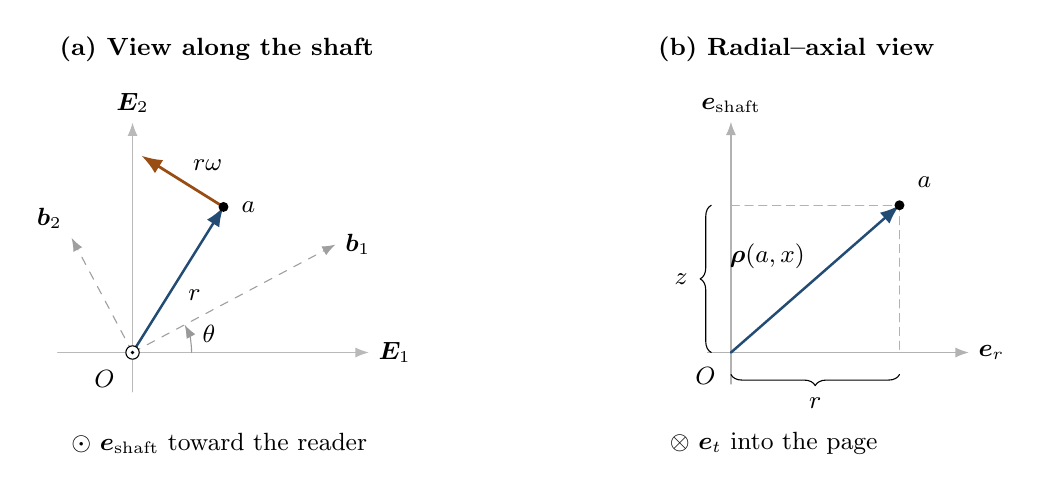
\begin{tikzpicture}[>=Latex, font=\small, line cap=round, line join=round]
  \begin{scope}[xshift=0.7cm,yshift=0.4cm]
    \node[anchor=west,font=\small\bfseries] at (-1.05,3.85) {(a) View along the shaft};
    \draw[gray!55,->] (-0.95,0) -- (3.00,0) node[right,text=black] {$\bm E_1$};
    \draw[gray!55,->] (0,-0.50) -- (0,2.92) node[above,text=black] {$\bm E_2$};
    \draw[gray!75,dashed,->] (0,0) -- (28:2.92) node[right,text=black] {$\bm b_1$};
    \draw[gray!75,dashed,->] (0,0) -- (118:1.65) node[above left,text=black] {$\bm b_2$};
    \draw[gray!80,->] (0.75,0) arc[start angle=0,end angle=28,radius=0.75];
    \node at (14:1.00) {$\theta$};
    \coordinate (A) at (58:2.18);
    \draw[vectorblue,line width=0.9pt,->] (0,0) -- (A) node[midway,below right,text=black] {$r$};
    \draw[vectororange,line width=1.0pt,->] (A) -- ++(148:1.23) node[midway,above right,text=black] {$r\omega$};
    \fill (A) circle (1.8pt);
    \node[right=3pt] at (A) {$a$};
    \draw[fill=white] (0,0) circle (0.085);
    \fill (0,0) circle (0.023);
    \node[below left=3pt] at (0,0) {$O$};
    \node[anchor=west] at (-0.90,-1.15) {$\odot\ \e$ toward the reader};
  \end{scope}
  \begin{scope}[xshift=8.3cm,yshift=0.4cm]
    \node[anchor=west,font=\small\bfseries] at (-1.05,3.85) {(b) Radial--axial view};
    \draw[gray!60,->] (-0.30,0) -- (3.02,0) node[right,text=black] {$\bm e_r$};
    \draw[gray!60,->] (0,-0.40) -- (0,2.93) node[above,text=black] {$\e$};
    \coordinate (B) at (2.14,1.87);
    \draw[gray!60,densely dashed] (0,1.87) -- (B) -- (2.14,0);
    \draw[vectorblue,line width=0.9pt,->] (0,0) -- (B) node[midway,above left,text=black] {$\rhoo(a,x)$};
    \draw[decorate,decoration={brace,mirror,amplitude=4pt}] (0,-0.28) -- (2.14,-0.28) node[midway,below=5pt] {$r$};
    \draw[decorate,decoration={brace,amplitude=4pt}] (-0.25,0) -- (-0.25,1.87) node[midway,left=5pt] {$z$};
    \fill (B) circle (1.8pt);
    \node[above right=3pt] at (B) {$a$};
    \node[below left=2pt] at (0,0) {$O$};
    \node[anchor=west] at (-0.90,-1.15) {$\otimes\ \bm e_t$ into the page};
  \end{scope}
\end{tikzpicture}
\caption{Position and shaft-induced velocity of one material point. In (a), the stationary Cartesian axes $\bm E_1,\bm E_2$ remain fixed while the dashed shaft-frame axes $\bm b_1,\bm b_2$ turn through $\theta$; the point is shown by its projection onto the transverse plane. The velocity arrow shows the contribution from positive shaft rotation at fixed $x$. In (b), the full position vector includes both radius $r$ and axial offset $z$. The tangential direction is normal to this radial--axial plane.}
\label{fig:coordinates}
\end{figure}

\FloatBarrier
\subsection{Notation and assumptions}

A dot denotes a time derivative. A prime denotes a derivative with respect to the local sheave coordinate $x$. Bold symbols are vectors or matrices. The principal notation is collected below; the inertia quantities are defined from the motion in \cref{sec:maps}.

\begin{center}
\renewcommand{\arraystretch}{1.13}
\begin{tabularx}{\textwidth}{@{}lX@{}}
\toprule
Symbol & Meaning\\
\midrule
$x,\dot x,\ddot x$ & Local sheave position, velocity, and acceleration\\
$\theta,\omega,\alpha$ & Shaft angle, angular velocity, and angular acceleration\\
$\mathcal F,\ a$ & Retained mechanism material and the label of one material point\\
$O,\ \e$ & Fixed origin on the shaft axis and its oriented axial unit vector\\
$r,z,\ \bm e_r,\bm e_t$ & Radial distance, axial position, and radial/tangential unit directions\\
$\rhoo(a,x),\ \bm y(a,t)$ & The origin-to-particle position in shaft and stationary coordinates\\
$R(\theta)$ & Rotation matrix converting shaft-frame to stationary-frame components\\
$\rhoo_x,\rhoo_{xx}$ & First and second position derivatives with respect to $x$, at fixed $a$\\
$M_f,\ M_f'$ & Effective mass for sheave motion and its position derivative\\
$J_f,\ J_f'$ & Shaft-axis inertia and its position derivative\\
$F_{f,x},\ \tau_f$ & Closing force and shaft reaction torque delivered by the mechanism\\
\bottomrule
\end{tabularx}
\end{center}

The reduction is made under the following local assumptions. They specify which motions and loads are represented, rather than a particular flyweight geometry.

\begin{enumerate}[label=\textbf{A\arabic*.},ref=A\arabic*,leftmargin=2.8em]
\item \label{ass:rigid}\textbf{Rigid hardware and a fixed shaft axis.}
The retained parts have prescribed rigid-body geometry and fixed mass properties in their own body frames. The shaft axis does not translate or tilt. This uses the rigid-hardware and fixed-axis setting of Assumptions 2 and 5 in \source.

\item \label{ass:branch}\textbf{One selected configuration branch.}
At each $x$ in the working interval, the active constraints determine the mechanism's internal positions and orientations. Holding the sheave and shaft fixed therefore holds the retained parts in one pose; a flyweight that can still swing freely would need an additional coordinate. The pose depends twice continuously differentiably on $x$. The selected contacts remain physically supportable; \cref{sec:admissibility} explains how branch validity and smoothness enter this requirement.

\item \label{ass:ideal}\textbf{Ideal transmission of the retained loads.}
The contact and guide constraints are frictionless. They can transmit forces and transfer work between connected parts without dissipating energy: their work on those parts cancels in a compatible motion. Additional actuator friction, backlash, compliance, and roller or pin spin are omitted, consistently with Assumption 3 of \source. The contribution derived here is inertial; springs and any other retained applied loads enter separately.

\item \label{ass:mixed}\textbf{No mixed shaft--shift kinetic term.}
If the shaft is held still while the sheave moves, the resulting mechanism motion carries no net angular momentum about the shaft. Entirely radial and axial motion satisfies this condition; opposite circumferential contributions can also cancel. Equivalently, the complete mechanism has no kinetic-energy term proportional to $\omega\dot x$. \Cref{sec:no-mixed} derives its coefficient and explains the cancellation. Axial pivot translation is allowed.
\end{enumerate}

Choose a fixed material set $\mathcal F$ containing the masses assigned to this mechanism. Each mass is counted once: material included here is excluded from the separate translating mass and fixed rotating inertia elsewhere in the pulley model. The same set is retained throughout the branch.

\section{From compatible motion to the inertia functions}
\label{sec:maps}

\subsection{The two contributions to a material point's velocity}
\label{sec:velocity}

The position description separates two physical motions. Changing $x$ moves a particle relative to the shaft; changing $\theta$ carries the configuration around the shaft. Differentiating \cref{eq:frame-position} at fixed material label $a$ makes both contributions explicit:
\begin{equation}
  \dot{\bm y}
    =R(\theta)\rhoo_x\dot x+\dot R(\theta)\rhoo,
  \qquad \rhoo_x=\frac{\partial\rhoo}{\partial x}.
  \label{eq:velocity-product-rule}
\end{equation}
The factor $\rhoo_x$ is the particle's displacement per unit sheave travel, so $\rhoo_x\dot x$ is its velocity relative to the shaft. The other term remains even when $x$ is fixed: the rotating axes carry the particle tangentially at speed $r\omega$. By \cref{eq:shaft-cross-radius}, that velocity has shaft-frame components $\omega\,\e\times\rhoo$. Converting them to stationary components gives
\begin{equation}
  \dot R(\theta)\rhoo
      =R(\theta)\left[\omega\,\e\times\rhoo\right].
  \label{eq:rotation-velocity}
\end{equation}
Substituting into \cref{eq:velocity-product-rule} therefore yields
\begin{equation}
  \dot{\bm y}
    =R(\theta)\left[\rhoo_x\dot x+\omega\,\e\times\rhoo\right].
  \label{eq:material-velocity}
\end{equation}
The bracket contains the \emph{total physical velocity expressed in shaft-frame components}. Only its first term is velocity relative to the shaft. Because both contributions belong to the same particle, its kinetic energy uses the squared length of their sum.

Rotations preserve vector lengths. Expanding that square and adding the energy of all retained mass gives
\begin{align}
  T_f
    &=\half\int_{\mathcal F}
      \left|\rhoo_x\dot x+\omega\,\e\times\rhoo\right|^2\dd m
      \notag\\
    &=\half M_f(x)\dot x^2+B_f(x)\omega\dot x
       +\half J_f(x)\omega^2,
       \label{eq:full-energy}
\end{align}
where
\begin{align}
  M_f(x)&=\int_{\mathcal F}|\rhoo_x|^2\dd m,
       \label{eq:M-definition}\\
  J_f(x)&=\int_{\mathcal F}|\e\times\rhoo|^2\dd m,
       \label{eq:J-definition}\\
  B_f(x)&=\int_{\mathcal F}\rhoo_x\cdot(\e\times\rhoo)\dd m.
       \label{eq:B-definition}
\end{align}
For a point-mass model, each integral is a sum over the retained masses. For finite rigid parts, Appendix~\ref{app:rigid} gives equivalent expressions using centres of mass and inertia tensors.

\term{Effective mass for sheave motion.}
$M_f$ measures how much mechanism motion accompanies a unit of sheave motion. If a point mass moves twice as fast as the sheave, its contribution to $M_f$ is four times its physical mass. If it does not move when $x$ changes, its contribution is zero. $M_f$ is consequently a mass referred to the coordinate $x$, and need not equal the mechanism's physical mass.

\term{Inertia for shaft rotation.}
$J_f$ is the ordinary mass moment of inertia about the shaft axis at the current configuration. For each material point, $|\e\times\rhoo|$ is its distance from that axis. The function changes when the mass distribution moves radially, even if the total mass is constant.

\needspace{11\baselineskip}
\subsection{When two functions are sufficient}
\label{sec:no-mixed}

The remaining coefficient $B_f$ couples the motion caused by shaft rotation to the motion caused by changing $x$. It comes from their cross term in the squared velocity. At one material point, the two velocity contributions have dot product
\begin{equation}
  (\rhoo_x\dot x)\cdot(\omega\,\e\times\rhoo)
  =\omega\dot x\,\rhoo_x\cdot(\e\times\rhoo).
  \label{eq:velocity-dot}
\end{equation}
If they point partly in the same direction, combining them increases the squared speed beyond the sum of their separate squared speeds. If they oppose one another, it decreases it. Perpendicular contributions have zero dot product and produce no cross term. Equation~\eqref{eq:B-definition} adds these signed contributions over the complete mechanism.

Shaft rotation gives a circumferential velocity. If a point's motion relative to the shaft is confined to a fixed radial--axial plane, its sheave-induced velocity is perpendicular to that circumferential direction. This is the plane used for the flyweight free body in Figure 3.6 of \source: it contains the shaft axis and the radial line to the point. Such a plane is also called a \emph{meridional plane} \cite{katsanis}. For example, a particle sliding both radially and axially in that plane has
\begin{equation}
  \rhoo_x=r_x\bm e_r+z_x\e,
  \qquad
  \rhoo_x\cdot(\e\times\rhoo)
     =(r_x\bm e_r+z_x\e)\cdot(r\bm e_t)=0.
  \label{eq:meridional-dot}
\end{equation}
Both sliding components belong to the motion driven by $x$; neither points along the shaft-induced tangential velocity. They contribute to $M_f$ through $|\rhoo_x|^2=r_x^2+z_x^2$, while their contribution to $B_f$ is zero. Relative circumferential motion can give a nonzero dot product.

A finite body need not have all its mass in one plane. The total $B_f$ also vanishes when its mass distribution and motion preserve reflection symmetry about a radial--axial plane: paired material points give equal and opposite dot products. Merely repeating identical components around the shaft does not, by itself, guarantee this cancellation.

Assumption~\ref{ass:mixed} therefore means
\begin{equation}
  B_f(x)\equiv0
  \quad\text{throughout the selected travel interval}.
  \label{eq:Bzero}
\end{equation}
The kinetic energy reduces to
\begin{equation}
  \boxed{T_f=\half M_f(x)\dot x^2+\half J_f(x)\omega^2.}
  \label{eq:reduced-energy}
\end{equation}
A pivot translating along the shaft adds axial motion to $\rhoo_x$. That motion is still perpendicular to the circumferential shaft velocity, so a translating pivot can change $M_f$ without introducing $B_f$. Its complete mass motion must be retained, but it need not require a third inertia function. Appendix~\ref{app:mixed} gives the additional force and torque terms when $B_f\ne0$.

\subsection{Why the derivatives require further geometric information}

The force balances will use the position derivatives of both inertia functions. Define
\begin{equation}
  \rhoo_{xx}=\frac{\partial^2\rhoo}{\partial x^2}
            =\frac{\partial\rhoo_x}{\partial x}.
  \label{eq:rho-xx}
\end{equation}
The subscript $xx$ means differentiation twice with respect to sheave position. It is not a component label or a time derivative. Whereas $\rhoo_x$ describes the point's displacement per unit sheave travel, $\rhoo_{xx}$ describes how that displacement ratio changes as the sheave moves.

The need for this second derivative follows directly from $M_f$. Its integrand is $\rhoo_x\cdot\rhoo_x$, so the product rule gives
\begin{equation}
  \frac{\partial}{\partial x}(\rhoo_x\cdot\rhoo_x)
  =\rhoo_{xx}\cdot\rhoo_x+\rhoo_x\cdot\rhoo_{xx}
  =2\rhoo_x\cdot\rhoo_{xx}.
\end{equation}
Differentiating over the fixed material set therefore yields
\begin{align}
  \boxed{M_f'(x)=2\int_{\mathcal F}
                \rhoo_x\cdot\rhoo_{xx}\dd m,}
       \label{eq:Mprime-definition}\\[0.3em]
  \boxed{J_f'(x)=2\int_{\mathcal F}
          (\e\times\rhoo)\cdot(\e\times\rhoo_x)\dd m.}
       \label{eq:Jprime-definition}
\end{align}
The same product rule gives the second expression, with the fixed axis vector $\e$ unchanged. Using the radial distance $r(a,x)$ defined in \cref{eq:position-components}, it can also be written
\begin{equation}
  J_f'=2\int_{\mathcal F}r\,r_x\dd m.
  \label{eq:Jprime-radial}
\end{equation}
Thus $M_f'$ requires second position derivatives because $M_f$ already depends on the first derivatives of the mass motion. In contrast, $J_f$ depends on position itself, so $J_f'$ requires only its first derivative.

\begin{center}
\begin{tabular}{@{}lll@{}}
\toprule
Quantity & Units & Mechanical role\\
\midrule
$M_f$ & $\mathrm{kg}$ & Inertia opposing sheave acceleration\\
$M_f'$ & $\mathrm{kg\,m^{-1}}$ & Variation of that inertia with travel\\
$J_f$ & $\mathrm{kg\,m^2}$ & Inertia opposing shaft acceleration\\
$J_f'$ & $\mathrm{kg\,m}$ & Centrifugal drive and shaft momentum transfer\\
\bottomrule
\end{tabular}
\end{center}

These are two functions and their derivatives, rather than four independently chosen laws. The same motion and mass distribution determine all four.

\section{The axial force delivered to the movable assembly}
\label{sec:axial}

Equation (3.2.1) of \source{} writes the primary movable-assembly balance as
\begin{equation}
  m_p\ddot x_p=F_{\mathrm{fw},x_p}
                  -F_{\mathrm{spring},x_p}-F_{\mathrm{belt},x_p}.
  \label{eq:paper-axial}
\end{equation}
Here $F_{\mathrm{fw},x_p}$ is the closing force supplied by the flyweights. In this note, $F_{f,x}$ denotes the corresponding contribution from the general centrifugal mechanism. For $x=x_p$, it occupies the same place in that balance; the spring and belt terms retain their meanings.

The meaning of the mechanism force must follow its attachments. In the paper's fixed-pivot arrangement, only the ramp contacts transmit axial work to the movable assembly, so the closing force is their axial resultant. If a pivot also moves with that assembly, its reaction can transmit work as well. We therefore define $F_{f,x}$ by the \emph{total} work delivered through all such connections:
\begin{equation}
  \delta W_{f\to\mathrm{sheave}}=F_{f,x}\,\delta x.
  \label{eq:force-work-definition}
\end{equation}
It is positive for a closing force. To evaluate this work, hold the shaft angle fixed and imagine a small sheave displacement $\delta x$ from the current configuration. Every mechanism part must follow its constraints during that displacement. This is a \emph{compatible virtual displacement}: it tests how forces act along the allowed motion, without advancing time or choosing an actual sheave speed.

\subsection{Centrifugal work}

That sheave displacement moves each material point by
\begin{equation}
  \delta\rhoo=\rhoo_x\,\delta x,
  \qquad \delta r=r_x\,\delta x.
  \label{eq:virtual-displacement}
\end{equation}
In the rotating frame, the point's centrifugal load is radial and outward, with magnitude $\omega^2r\,\dd m$. Only the radial component $\delta r$ of its displacement contributes to this load's virtual work. The force--displacement product for one mass element is therefore $(\omega^2r\,\dd m)\delta r$. Adding all the elements gives
\begin{align}
  \delta W_{f,\mathrm{cent}}
    &=\int_{\mathcal F}\omega^2r\,\delta r\,\dd m
      =\omega^2\int_{\mathcal F}r\,r_x\dd m\,\delta x
      \notag\\
    &=\half\omega^2J_f'(x)\,\delta x.
      \label{eq:centrifugal-work}
\end{align}
The final equality uses the radial-inertia derivative in \cref{eq:Jprime-radial}, with instantaneous $\omega$ held fixed during the virtual displacement. This recovers the work identity used in Equation (3.2.6) of \source{}. Centrifugal loading pushes each mass outward. When closing lets the masses move outward, it assists closure; when closing draws them inward, it opposes closure. The derivative $J_f'$ adds the contributions of all retained mass and determines the net closing or opening tendency.

\subsection{The loading retained to accelerate the mechanism}

Some of the centrifugal drive is needed to accelerate the mechanism's own motion. Differentiating its relative velocity $\rhoo_x\dot x$ gives
\begin{equation}
  \bm a_{\mathrm{rel}}
    =\frac{\dd}{\dd t}(\rhoo_x\dot x)
    =\rhoo_x\ddot x+\rhoo_{xx}\dot x^2.
  \label{eq:relative-acceleration}
\end{equation}
The first term is caused by sheave acceleration. The second accounts for the changing internal velocity as the mechanism traverses its path. Even at constant sheave speed, a changing motion ratio can make a flyweight rotate progressively faster or slower, so its inertia still requires a load. This is the same effect identified in Equation (3.2.9) of \source.

For a mass element $\dd m$, the corresponding mass-times-acceleration demand is $\bm a_{\mathrm{rel}}\,\dd m$. Project it onto the compatible displacement in \cref{eq:virtual-displacement}, using the acceleration from \cref{eq:relative-acceleration}:
\begin{align}
  \delta W_{f,\mathrm{acc}}
    &=\int_{\mathcal F}\bm a_{\mathrm{rel}}\cdot\delta\rhoo\,\dd m
        \notag\\
    &=\int_{\mathcal F}
       \left(\rhoo_x\ddot x+\rhoo_{xx}\dot x^2\right)
        \cdot\rhoo_x\,\dd m\,\delta x
        \notag\\
    &=\left[M_f\ddot x+\half M_f'\dot x^2\right]\delta x.
       \label{eq:acceleration-work}
\end{align}
The last line uses $M_f$ and $M_f'$ from \cref{eq:M-definition,eq:Mprime-definition}. The dot product is the force--displacement product for vectors that need not be parallel. This expression is the virtual-work form of the inertial demand, rather than another applied load or a finite change in stored energy.

The rotating frame also introduces Coriolis and shaft-angular-acceleration terms. The Coriolis term has zero projection because
$\rhoo_x\cdot(\e\times\rhoo_x)=0$.
The shaft-angular-acceleration term projects to $B_f\alpha$, which is zero under \cref{eq:Bzero}. No omitted $\alpha$ contribution is therefore hidden in \cref{eq:acceleration-work}; Appendix~\ref{app:mixed} shows where it enters when $B_f\ne0$.

\subsection{The force entering the sheave balance}

Ideal internal constraint forces transfer work between the connected parts without dissipating it. Their internal contributions cancel, and a support that does not move with $x$ contributes no work to this displacement. The centrifugal work remaining after the mechanism's inertial demand is supplied is therefore delivered to the movable assembly. Substituting \cref{eq:centrifugal-work,eq:acceleration-work} into this work balance gives
\begin{align}
  F_{f,x}\delta x
     &=\delta W_{f,\mathrm{cent}}-\delta W_{f,\mathrm{acc}}
       \notag\\
     &=\left[\half J_f'\omega^2-M_f\ddot x
                    -\half M_f'\dot x^2\right]\delta x.
       \label{eq:assembled-work}
\end{align}
Both sides now contain the same factor $\delta x$. Cancelling it gives
\begin{equation}
  \boxed{F_{f,x}
     =\half J_f'(x)\omega^2
      -M_f(x)\ddot x-\half M_f'(x)\dot x^2.}
  \label{eq:force}
\end{equation}

The first term is the centrifugal closing drive. The second is the force retained to accelerate the internal motion accompanying sheave acceleration. The third accounts for the changing motion ratio as the mechanism traverses its path. This last term is inertial, not a damping force: it does not change sign simply because $\dot x$ changes sign, and its sign depends on $M_f'$.

For the primary, substitute \cref{eq:force} into \cref{eq:paper-axial} with $x=x_p$, and collect the terms multiplying $\ddot x_p$ on the left:
\begin{equation}
  \boxed{[m_p+M_f(x_p)]\ddot x_p
      =\half J_f'(x_p)\omega_p^2-\half M_f'(x_p)\dot x_p^2
       -F_{\mathrm{spring},x_p}-F_{\mathrm{belt},x_p}.}
  \label{eq:completed-axial}
\end{equation}
The remaining loads are still those of Equations (3.2.12)--(3.2.13) of \source:
\begin{equation}
  F_{\mathrm{spring},x_p}=k_p(x_{p,\mathrm{pre}}+x_p),
  \qquad
  F_{\mathrm{belt},x_p}=\frac{N_p}{2}\cos\beta.
\end{equation}
Here $k_p$ is spring stiffness, $x_{p,\mathrm{pre}}$ is installed compression, $N_p$ is the integrated normal load over both primary faces, and $\beta$ is their half-angle measured from the radial direction. The separate translating mass $m_p$ excludes all material already represented by $M_f$.

\section{The reaction on the shaft}
\label{sec:shaft}

Section 3.3.2 of \source{} accounts for the flyweights through their angular momentum about the primary shaft. Generalizing their internal motion requires the same accounting. The centrifugal closing force and the shaft reaction come from the same moving mass.

For one mass element, angular momentum about the shaft is $r\,v_t\,\dd m$, where $v_t$ is its signed tangential velocity. Motion directly outward or along the shaft contributes no angular momentum about that axis. By \cref{eq:shaft-cross-radius}, the vector $\e\times\rhoo=r\bm e_t$ contains both the radius and the tangential direction. Its dot product with the total velocity therefore selects exactly $r\,v_t$. Using the velocity in \cref{eq:material-velocity} and summing over the retained mass gives
\begin{align}
  H_f
    &=\int_{\mathcal F}
       (\e\times\rhoo)\cdot
       \left(\rhoo_x\dot x+\omega\,\e\times\rhoo\right)\dd m
       \notag\\
    &=B_f\dot x+J_f\omega.
      \label{eq:full-momentum}
\end{align}
The second line uses the definitions of $B_f$ and $J_f$ in \cref{eq:B-definition,eq:J-definition}. If the shaft is held still, $\omega=0$ and the remaining angular momentum is $B_f\dot x$. This makes the physical meaning of Assumption~\ref{ass:mixed} explicit: the sheave-induced motion carries no net angular momentum about the shaft. With $B_f=0$, \cref{eq:full-momentum} and its time derivative reduce to
\begin{equation}
  H_f=J_f(x)\omega,
  \qquad
  \dot H_f=J_f\alpha+J_f'\dot x\omega.
  \label{eq:momentum}
\end{equation}
Changing shaft speed requires the first torque. The second is required when the mass distribution changes while the shaft turns. In an otherwise isolated rotating assembly, moving mass outward increases its inertia and lowers its speed. Maintaining the same $\omega$ instead requires additional angular momentum from the drive. This is the mechanism contribution differentiated in Equations (3.3.3)--(3.3.4) of \source.

Let $\tau_f$ be the torque exerted by the mechanism on the shaft and its attached carrier. The torque supplied to accelerate the mechanism has the opposite sign, so
\begin{equation}
  \boxed{\tau_f=-J_f(x)\alpha-J_f'(x)\dot x\omega.}
  \label{eq:torque}
\end{equation}
This reaction must accompany the axial force in \cref{eq:force}. Thus $B_f=0$ still allows shaft rotation to drive closure and shifting to alter the shaft motion through the changing $J_f(x)$. Both exchanges arise from the same radial mass redistribution and must be retained together.

Using the primary balance conventions of \source{}, let $I_{B,p}$ be the fixed equivalent inertia of the attached system, $I_{p,\mathrm{const}}$ the separately represented constant primary inertia, $\tau_{B,p}$ the applied boundary torque, and $\tau_p$ the signed belt torque on the primary. Then
\begin{equation}
  \tau_{B,p}+\tau_p
    =[I_{B,p}+I_{p,\mathrm{const}}+J_f(x_p)]\dot\omega_p
      +J_f'(x_p)\dot x_p\omega_p.
  \label{eq:completed-rotation}
\end{equation}
For $x_p=s$, this is the structure of Equation (3.3.5) of \source. Generalizing the internal kinematics changes the inertia functions supplied to that balance, not the angular-momentum principle behind it.

\section{Admissible motion and smoothness}
\label{sec:admissibility}

The four quantities are now defined and their dynamic roles established. To use them over a finite travel interval, the underlying motion must remain a valid function of $x$, and its derivatives must remain suitable for the force and torque calculations.

\subsection{How contact geometry determines a local motion}
\label{sec:geometry}

A mechanism usually begins with geometric constraints, rather than an explicit position map $\rhoo(a,x)$. At a specified sheave position, an arm angle or a contact location must adjust so that those constraints remain satisfied.

First consider one internal variable $u$ determined by one smooth constraint,
\begin{equation}
  \phi(u,x)=0.
\end{equation}
A small change in $x$ changes the constraint residual by $\phi_x\,\dd x$. Changing $u$ can compensate by $\phi_u\,\dd u$. Remaining on the constraint requires
\begin{equation}
  \phi_u\,\dd u+\phi_x\,\dd x=0,
  \qquad
  u'=-\frac{\phi_x}{\phi_u},
  \quad \phi_u\ne0.
  \label{eq:scalar-implicit}
\end{equation}
The subscripts on $\phi$ denote partial derivatives with the other variable held fixed. A nonzero $\phi_u$ makes the required local adjustment possible and determines its motion ratio. This is the scalar construction used for the roller-contact location in Appendix A.2 of \source.

With several internal variables and constraints, the same statement becomes a linear system. Write the internal variables as a vector $\bm u$ and the geometric constraints as $\bm\Phi(\bm u,x)=\bm0$. Then
\begin{equation}
  \bm\Phi_{\bm u}\,\bm u'=-\bm\Phi_x,
  \qquad
  (\bm\Phi_{\bm u})_{ij}=\frac{\partial\Phi_i}{\partial u_j}.
  \label{eq:implicit-first}
\end{equation}
The matrix $\bm\Phi_{\bm u}$ is the \emph{constraint Jacobian}: each entry tells how one constraint changes when one internal variable changes. For an equal number of independent constraints and internal variables, an invertible Jacobian gives a unique solution for this local motion ratio.

More precisely, at a solution of sufficiently smooth constraints, this invertibility guarantees a unique nearby function $\bm u(x)$ through the chosen configuration. This is the implicit function theorem \cite{implicit}. It is a local result; other assembled configurations may exist elsewhere. The selected branch must be continued across the intended interval. Differentiating the constraints once more supplies $\bm u''$ and hence the second position derivatives needed by $M_f'$; Appendix~\ref{app:constraints} gives those steps.

If the Jacobian becomes singular, this guarantee is lost. A small sheave displacement may demand a very large internal motion, or $x$ may cease to determine the configuration. Large or divergent $M_f$ can then reflect a failing branch or coordinate, rather than a force that should be continued by clipping its value.

Geometric solvability is only part of retaining that branch. A contact assumed to remain closed must also support its required reaction. A roller can push against a ramp, but a one-sided contact cannot pull the surfaces together. With compression taken as positive, the required normal reaction must therefore remain nonnegative. The ideal-work reduction eliminates the individual reactions, so the four inertia quantities do not establish this condition by themselves. In particular, the paper's fixed-pivot check $F_{\mathrm{fw},x_p}\ge0$ does not automatically apply to a net force that also includes a moving-pivot reaction. The working interval must respect the chosen mechanism's contact conditions as well as its geometry. If contact loss frees an internal motion, that motion needs its own dynamic coordinate rather than continuation of the same map.

\subsection{Regularity of the motion and the reduced functions}

At the reduced boundary, continuous force and torque require finite, mutually consistent values of $M_f$, $M_f'$, $J_f$, and $J_f'$. A natural minimum is
\begin{equation}
  M_f,J_f\in C^1,
  \label{eq:C1}
\end{equation}
meaning that each function and its first derivative are continuous. At physical interval endpoints, the corresponding one-sided limits must be finite. At an interior interpolation junction, values and derivatives must agree across the junction if the same smooth branch continues through it. Otherwise, joining two approximations can introduce an artificial jump in the predicted force or torque even though the physical motion remains smooth.

For finitely many rigid bodies, twice continuously differentiable position maps are sufficient to construct these quantities, as assumed in Assumption~\ref{ass:branch}.\footnote{For a general distributed-mass integral, the derivatives must also be bounded appropriately over the retained mass so that differentiation can pass under the integral.} This follows from \cref{eq:M-definition,eq:Mprime-definition,eq:J-definition,eq:Jprime-definition}: the highest position derivative used is $\rhoo_{xx}$. It is a sufficient construction condition, not a requirement to represent every mechanism in the same geometric variables.

The underlying contact profile can require more derivatives. In the finite-roller construction of Appendix A.2.1 of \source{}, the contact normal already uses the ramp slope $h'$. Differentiating the resulting position map twice brings in $h'''$, giving the stated $h\in C^3$ requirement in Equation (A.2.12). This is a requirement of that geometry construction; a directly supplied $M_f$ or $J_f$ does not universally need three derivatives.

Continuity of these forces is distinct from uniqueness of the time evolution. A convenient stronger condition is that the first derivatives of $M_f$ and $J_f$ are locally Lipschitz: on a small interval, their changes are bounded by a constant times the change in $x$. With corresponding regularity of the other terms and a nonsingular coupled closure, this supports the usual local uniqueness result for a continuous regime. This condition is often written $C^{1,1}_{\mathrm{loc}}$.

\subsection{Consistency of the four quantities}

By construction, $M_f\ge0$ and $J_f\ge0$. Neither has to be strictly positive everywhere; the assembled dynamics must remain solvable. Their derivatives can have either sign. In particular, $J_f'>0$ gives a centrifugal closing tendency, whereas $J_f'<0$ gives an opening tendency under the present coordinate convention.

The two inertia functions are also linked by their common mass motion. Applying the Cauchy--Schwarz inequality to \cref{eq:Jprime-definition}, and using $|\e\times\rhoo_x|\le|\rhoo_x|$, gives
\begin{equation}
  (J_f')^2\le4J_fM_f.
  \label{eq:map-consistency}
\end{equation}
A mass distribution cannot change its shaft inertia with $x$ while requiring no mass motion in that coordinate. This is a necessary check on maps derived from the retained material, not a proof that a proposed geometry and its contacts are feasible.

Each derivative must come from the same geometry or interpolant as its parent function. A static centrifugal-force curve can determine $J_f'$ through $F_{f,x}=\half J_f'\omega^2$ when $\dot x=\ddot x=0$. It does not determine $M_f$ or the additive constant in $J_f$, both of which affect the transient response. Two mechanisms can therefore produce the same steady clamping force yet require different torques during shaft acceleration and different axial forces during shifting. The transient boundary needs their motion and mass information as well as the static force curve.

\section{The boundary supplied to the transient model}
\label{sec:interface}

The mechanism supplies $M_f$, $M_f'$, $J_f$, and $J_f'$ at the current local sheave position, on its stated valid branch. The surrounding model uses these quantities in both the continuous balances and the momentum calculations at events.

\subsection{Continuous force and torque}

At known $x$, $\dot x$, and $\omega$, the only unknowns in \cref{eq:force,eq:torque} are the accelerations. They enter linearly: $-M_f$ multiplies $\ddot x$ in the closing force, and $-J_f$ multiplies $\alpha$ in the shaft reaction. The remaining terms are known at that state.

This is the affine form used by CINDER's coupled closure: the mechanism supplies these coefficients to the same solve that determines the current accelerations.

\subsection{Local sheave motion and the shared shift coordinate}
\label{sec:coordinate}

The primes in this note differentiate with respect to $x$. If the system advances a shared coordinate $s$, let the local sheave position be $x=\chi(s)$. The chain rule gives
\begin{equation}
  \dot x=\chi_s\dot s,
  \qquad
  \ddot x=\chi_s\ddot s+\chi_{ss}\dot s^2,
  \label{eq:chain-rule}
\end{equation}
where $\chi_s=\dd\chi/\dd s$ and $\chi_{ss}=\dd^2\chi/\dd s^2$. Section 3.2.3 of \source{} uses these local-to-shared relations; for the primary, $x_p=s$.

Substitute \cref{eq:chain-rule} into the local force and torque laws, \cref{eq:force,eq:torque}, before assembling the balances. A further factor appears only if the force itself is projected onto the shared coordinate. Equality of virtual work gives
\begin{equation}
  F_{f,s}\delta s=F_{f,x}\delta x,
  \qquad F_{f,s}=\chi_sF_{f,x}.
  \label{eq:shared-force}
\end{equation}
Consequently the effective mass in a generalized equation for $s$ is
\begin{equation}
  M_{f,s}(s)=M_f(\chi(s))\chi_s^2.
  \label{eq:shift-mass}
\end{equation}
The square reflects both the local motion ratio and the force projection. A local sheave balance uses $F_{f,x}$, so it receives the acceleration substitution but not this additional force-projection factor. These relations apply on each smooth geometric branch.

\subsection{The same inertia at an event}
\label{sec:events}

Section 3.6 of \source{} treats finite-speed constraint activation through momentum balance. When a travel stop arrests the sheave, it also arrests the relative mechanism motion tied to that travel. The mechanism's moving mass must therefore take part in the momentum calculation. The same accounting applies when a retained belt constraint changes a velocity.

At the event position, the kinetic energy in \cref{eq:reduced-energy} contributes
\begin{center}
\begin{tabular}{@{}llll@{}}
\toprule
Motion & Inertia & Speed & Kinetic energy\\
\midrule
Shaft rotation & $J_f(x)$ & $\omega$ & $\half J_f\omega^2$\\
Sheave motion & $M_f(x)$ & $\dot x$ & $\half M_f\dot x^2$\\
\bottomrule
\end{tabular}
\end{center}
In shared coordinates the second speed is $\chi_s\dot s$, giving the same $M_f\chi_s^2$ contribution as \cref{eq:shift-mass}. The map values supply the instantaneous inertia used in the momentum calculation. Their derivatives supply the continuous velocity-dependent terms; they are not additional impulsive inertia coefficients.

This description applies while the actuator retains the same physical velocity mapping across the event. If the actuator's own contact arrangement changes, the transition also needs the compatible material velocities and the new constraints. The four scalar quantities alone do not determine momentum transfer between different actuator branches. An inelastic impact may lose kinetic energy even though the intervening smooth, ideal motion satisfies the power identity derived next.

\needspace{28\baselineskip}
\section{A final energy check}
\label{sec:energy}

The axial and shaft contributions describe two exchanges with the same mechanism. Their combined power should therefore account for the change in its retained kinetic energy. Differentiating \cref{eq:reduced-energy} gives
\begin{equation}
  \frac{\dd T_f}{\dd t}
   =M_f\dot x\ddot x+\half M_f'\dot x^3
     +J_f\omega\alpha+\half J_f'\dot x\omega^2.
  \label{eq:energy-derivative}
\end{equation}
Now multiply \cref{eq:force} by $\dot x$ and \cref{eq:torque} by $\omega$, then add:
\begin{equation}
  \boxed{F_{f,x}\dot x+\tau_f\omega
          =-\frac{\dd T_f}{\dd t}.}
  \label{eq:power}
\end{equation}
The left side is the power delivered by the mechanism to its surroundings. Its negative is the rate at which the mechanism stores kinetic energy. This identity checks the force sign, torque sign, and the factors of one half together.

The different coefficients of $J_f'$ in the force and torque are necessary. At constant shaft speed, increasing $J_f$ requires shaft power $J_f'\dot x\omega^2$. Half increases the rotational kinetic energy $\half J_f\omega^2$; the other half appears as the centrifugal contribution to sheave power. The complete sheave power also accounts for the changing kinetic energy of the relative motion through the $M_f$ terms.

The four-quantity boundary therefore joins the two balances through one consistent kinetic energy. A change to the mechanism's motion changes the functions supplied at that boundary; the axial force, shaft reaction, and event inertia must all use those same functions.


\clearpage
\section{Canonical CINDER implementation}
\label{sec:canonical}

CINDER 1.2.0 implements this boundary in
\texttt{cinder.model.cvt.actuation}. The immutable record
\texttt{CentrifugalInertiaSample} contains \texttt{effective\_mass},
\texttt{effective\_mass\_gradient}, \texttt{shaft\_inertia}, and
\texttt{shaft\_inertia\_gradient}, in the order of the four quantities derived
above. A \texttt{CentrifugalInertiaMap} supplies that record through
\texttt{evaluate(x)} and declares \texttt{axial\_position\_min} and
\texttt{axial\_position\_max}.

\texttt{CentrifugalInertiaForce} is the single common implementation of the
closing force, owning-shaft reaction, inspected force terms, and two kinetic
modes. Its host supplies the full affine local acceleration, including any
curvature bias from the shared shift coordinate. The same kinetic modes enter
stored energy and event projection; a mechanism does not add its inertia to
those calculations a second time.

The fixed-pivot provider adapts its existing angle and mass-moment map. The
sliding-block provider constructs the four quantities from a compiled COM
translation and a centroidal tensor. Their companion documents are
\href{../fixed_pivot/formulation.pdf}{Fixed-Pivot Roller Flyweights} and
\href{../sliding_block/formulation.pdf}{Fixed-Orientation Sliding Blocks}.
The common evaluator owns the dynamics in both cases; each mechanism owns its
contact conditions and geometric domain. CINDER 1.2.1 extends the sliding-block
contact construction to point-defined and piecewise polynomial profiles and
common-normal contact sets. Those geometry choices do not alter the boundary
relations derived here. Saved documents retain physical
geometry and mass properties, rather than independent fits of four functions.

A kinetic projection is a candidate velocity reset, not a contact-feasibility
proof. Mechanisms may expose the normal impulses required by that candidate.
The sliding-block implementation supplies both named contact impulses and the
ideal guide impulse; a selected hybrid reset is rejected if a retained contact
would require tension. The generic projection API exposes these margins and
provides \texttt{require\_admissible\_mechanism\_impulses()} for direct callers.
This addition does not implement release, flight, rocking, or recontact.

\clearpage
\appendix
\section{When the mixed kinetic term does not vanish}
\label{app:mixed}
\noindent{\small\hyperref[sec:no-mixed]{Return to Section~\ref*{sec:no-mixed}: when two functions are sufficient.}}\par

Assumption~\ref{ass:mixed} is the condition that reduces the boundary to $M_f$ and $J_f$ with their derivatives. If it does not hold, retain the full kinetic energy:
\begin{equation}
  T_f=\half M_f\dot x^2+B_f\omega\dot x+\half J_f\omega^2.
  \label{eq:mixed-energy}
\end{equation}
The complete stationary-frame acceleration corresponding to \cref{eq:material-velocity} is
\begin{align}
  \ddot{\bm y}=R(\theta)\big[&
      \rhoo_x\ddot x+\rhoo_{xx}\dot x^2
      +2\omega\dot x\,\e\times\rhoo_x\notag\\
      &+\alpha\,\e\times\rhoo
      +\omega^2\e\times(\e\times\rhoo)\big].
      \label{eq:full-acceleration}
\end{align}
These are, respectively, relative acceleration, Coriolis acceleration, shaft-angular-acceleration, and centripetal acceleration terms.

Project the bracketed acceleration in \cref{eq:full-acceleration} along $\rhoo_x$, the material displacement per unit sheave travel from \cref{eq:virtual-displacement}. Integrating over mass and using the definitions of $M_f$, $M_f'$, $B_f$, and $J_f'$ in \cref{eq:M-definition,eq:Mprime-definition,eq:B-definition,eq:Jprime-definition} gives the generalized inertial demand
\begin{equation}
  M_f\ddot x+\half M_f'\dot x^2+B_f\alpha-\half J_f'\omega^2.
\end{equation}
The Coriolis projection is zero because its direction is perpendicular to $\rhoo_x$. The shaft-angular-acceleration term contributes $B_f\alpha$; the centripetal term supplies the negative of the centrifugal drive. The force delivered to the sheave is the opposite of this demand:
\begin{equation}
  \boxed{F_{f,x}=\half J_f'\omega^2-M_f\ddot x
                  -\half M_f'\dot x^2-B_f\alpha.}
  \label{eq:mixed-force}
\end{equation}

The shaft-axis angular momentum is now the full expression in \cref{eq:full-momentum}, $H_f=J_f\omega+B_f\dot x$. Differentiating it and taking the opposite sign for the reaction on the shaft gives
\begin{equation}
  \boxed{\tau_f=-J_f\alpha-J_f'\dot x\omega
                     -B_f\ddot x-B_f'\dot x^2.}
  \label{eq:mixed-torque}
\end{equation}
The same coefficient $B_f$ couples shaft acceleration into the axial force and sheave acceleration into the shaft torque. Their common origin is the symmetric kinetic matrix
\begin{equation}
  \begin{bmatrix}M_f&B_f\\B_f&J_f\end{bmatrix},
  \qquad M_f\ge0,\quad J_f\ge0,\quad M_fJ_f-B_f^2\ge0.
\end{equation}
The inequalities follow from kinetic energy being nonnegative for every pair $(\dot x,\omega)$. They constrain the mechanism contribution; the complete system must still be nonsingular on its independent velocities.

Including the mixed terms preserves
\begin{equation}
  F_{f,x}\dot x+\tau_f\omega=-\frac{\dd T_f}{\dd t}.
\end{equation}
Thus a nonzero $B_f$ requires additional boundary data, $B_f$ and $B_f'$. It cannot be absorbed into independently modified $M_f$ and $J_f$ while retaining the four-quantity force and torque laws.

\clearpage
\section{Derivatives of an implicitly defined motion}
\label{app:constraints}
\noindent{\small\hyperref[sec:geometry]{Return to Section~\ref*{sec:geometry}: contact geometry and local motion.}}\par

For the constraints $\bm\Phi(\bm u,x)=\bm0$, \cref{eq:implicit-first} gives the first-derivative relation
\begin{equation}
  \bm\Phi_{\bm u}\bm u'=-\bm\Phi_x.
\end{equation}
Here we obtain the second derivative needed to construct $\rhoo_{xx}$ and $M_f'$. All partial derivatives below hold the other arguments fixed; primes follow the selected branch $\bm u(x)$.

For one internal variable, differentiate \cref{eq:scalar-implicit} in its undivided form:
\begin{equation}
  \phi_u u''+\phi_{uu}(u')^2+2\phi_{ux}u'+\phi_{xx}=0.
\end{equation}
Thus
\begin{equation}
  u''=-\frac{\phi_{xx}+2\phi_{ux}u'+\phi_{uu}(u')^2}{\phi_u}.
\end{equation}
The same nonzero denominator is required as for $u'$. This is the scalar second-derivative construction used in Equation (A.2.5) of \source.

For several variables, differentiate row $i$ of \cref{eq:implicit-first} along the selected branch and collect the terms multiplying $\bm u''$:
\begin{equation}
  \sum_j\frac{\partial\Phi_i}{\partial u_j}\,u_j''
   =-\left[
       \frac{\partial^2\Phi_i}{\partial x^2}
       +2\sum_j\frac{\partial^2\Phi_i}{\partial x\,\partial u_j}u_j'
       +\sum_{j,k}
         \frac{\partial^2\Phi_i}{\partial u_j\,\partial u_k}u_j'u_k'
     \right].
  \label{eq:implicit-second}
\end{equation}
Every quantity on the right is known from the configuration and its first derivative. The coefficient matrix on the left is again the constraint Jacobian, so solving this linear system gives $\bm u''$.

Finally, suppose a material position is first written in terms of these internal variables as $\widehat{\rhoo}(a,\bm u,x)$. Its branch value is $\rhoo(a,x)=\widehat{\rhoo}(a,\bm u(x),x)$. Applying the chain rule gives
\begin{align}
  \rhoo_x
    &=\widehat{\rhoo}_x+\sum_j\widehat{\rhoo}_{u_j}u_j',
      \label{eq:position-first}\\
  \rhoo_{xx}
    &=\widehat{\rhoo}_{xx}
      +2\sum_j\widehat{\rhoo}_{x u_j}u_j'
      +\sum_{j,k}\widehat{\rhoo}_{u_j u_k}u_j'u_k'
      +\sum_j\widehat{\rhoo}_{u_j}u_j''.
      \label{eq:position-second}
\end{align}
On the right, the subscripts are partial derivatives of $\widehat{\rhoo}$ before imposing the constraints. On the left, they are derivatives of the resulting position map along the selected motion. Substitution into \cref{eq:M-definition,eq:J-definition,eq:Mprime-definition,eq:Jprime-definition} supplies the four boundary quantities from the same constrained geometry.

\clearpage
\section{Computing the maps from rigid-body mass properties}
\label{app:rigid}
\noindent{\small\hyperref[sec:velocity]{Return to Section~\ref*{sec:velocity}: velocity and inertia definitions.}}\par

The material integrals are a definition, not a requirement to discretize a solid into point masses. For a collection of rigid bodies, the same quantities can be obtained from their masses, centres of mass, inertia tensors, and poses.

For body $k$, let $m_k$ be its mass, $\bm g_k(x)$ its centre-of-mass position in the shaft frame, and $\bm I_{C,k}(x)$ its centroidal inertia tensor expressed in that frame. Let $\bm\kappa_k(x)$ be its relative angular velocity per unit sheave speed, so that its angular velocity relative to the shaft frame is $\bm\kappa_k\dot x$. All primes in this appendix denote total derivatives with respect to $x$ along the selected branch.

The centre-of-mass velocity, expressed in the shaft frame, is
$\bm g_k'\dot x+\omega\,\e\times\bm g_k$.
The body's absolute angular velocity in the same frame is
$\bm\kappa_k\dot x+\omega\e$.
Expanding the translational and rotational kinetic energies gives
\begin{align}
  M_f&=\sum_k\left[m_k|\bm g_k'|^2
                  +\bm\kappa_k^{T}\bm I_{C,k}\bm\kappa_k\right],
                  \label{eq:body-M}\\
  J_f&=\sum_k\left[m_k|\e\times\bm g_k|^2
                         +\e^{T}\bm I_{C,k}\e\right],
                         \label{eq:body-J}\\
  B_f&=\sum_k\left[m_k\bm g_k'\cdot(\e\times\bm g_k)
                         +\bm\kappa_k^{T}\bm I_{C,k}\e\right].
                         \label{eq:body-B}
\end{align}
The first part of $M_f$ is centre-of-mass translation, and the second is relative rotation about the centre. The two parts of $J_f$ are the parallel-axis contribution and the centroidal inertia projected onto the shaft axis. The formula for $B_f$ allows its cancellation to be checked from the body data.

Differentiating \cref{eq:body-M,eq:body-J} gives
\begin{align}
  M_f'&=\sum_k\left[2m_k\bm g_k'\cdot\bm g_k''
      +2(\bm\kappa_k')^T\bm I_{C,k}\bm\kappa_k
      +\bm\kappa_k^T\bm I_{C,k}'\bm\kappa_k\right],
      \label{eq:body-Mprime}\\
  J_f'&=\sum_k\left[2m_k(\e\times\bm g_k)\cdot
                           (\e\times\bm g_k')
                    +\e^T\bm I_{C,k}'\e\right].
                    \label{eq:body-Jprime}
\end{align}
For a rigid body, the centroidal inertia is constant in a body-fixed frame, but generally changes when expressed in the shaft frame. Turning the body can change its material points' distances from the shaft even when its centre of mass stays fixed. If $Q_k(x)$ maps that body frame into the shaft frame, use
\begin{equation}
  \bm I_{C,k}=Q_k\bm I_{C,k}^{\mathrm{body}}Q_k^T,
  \qquad
  Q_k'Q_k^T\bm v=\bm\kappa_k\times\bm v
  \quad\text{for any vector }\bm v.
\end{equation}
These relations determine the orientation derivatives consistently. In particular, an orientation-dependent shaft-axis inertia must not be replaced by a constant centroidal scalar unless the body's geometry and motion justify it.

The centre-of-mass path includes any pivot translation and its interaction with relative body rotation. Constructing the maps from this complete pose therefore retains both motions without adding a separate inertial correction afterward.

\clearpage
\begingroup
\raggedright
\begin{thebibliography}{9}
\addcontentsline{toc}{section}{References}
\bibitem{formulation}
Kai Arseneau and W. Spencer Smith.
\emph{A First-Principles Dynamic Model of a Rubber V-Belt CVT for General Transient Simulation: With Mechanical Actuation and Traction-Limited Torque Transfer}.
Manuscript supplied with this work, October 1, 2026.
Relevant locations: Sections 2.2--2.3 (assumptions and coordinate conventions), Section 3.2.1 (primary actuation), Section 3.2.3 (shared shift coordinate), Section 3.3.2 (primary angular momentum), Section 3.6 (contact and support transitions), and Appendix A (fixed-pivot geometry and mass properties).

\bibitem{katsanis}
Theodore Katsanis.
\emph{Use of Arbitrary Quasi-Orthogonals for Calculating Flow Distribution in the Meridional Plane of a Turbomachine}.
NASA Technical Note D-2546, December 1964, pp.~2--3.
The meridional plane is defined as a plane containing the rotation axis.
\href{https://ntrs.nasa.gov/api/citations/19650002705/downloads/19650002705.pdf}{NASA report}.

\bibitem{implicit}
MIT OpenCourseWare.
\emph{18.994 Seminar in Geometry}, Fall 2004.
Lecture notes, Chapter 4, \emph{Implicit Function Theorem}, Theorem 4.1.1.
\href{https://ocw.mit.edu/courses/18-994-seminar-in-geometry-fall-2004/6e9f9f4820f735f233f28531a3a43a3a_chapter4.pdf}{Course notes}.
\end{thebibliography}
\endgroup
\end{document}
